\section{CPU scheduler}
Abbiamo visto in 2.3.1 il lifecycle di un processo, lo scheduler della CPU deve prendere una decisione in queste situazioni:
\begin{enumerate}
    \item \textbf{Suspend:} Avviene principalmente come risultato di una richiesta di I/O, è quindi richiesto dal processo stesso.
    \item \textbf{Resign:} Il processo viene forzatamente interrotto dallo scheduler.
    \item \textbf{Resume:} La condizione attesa diventa vera e il processo è pronto ad utilizzare nuovamente risorse di sistema.
    \item \textbf{Termina}
\end{enumerate}

Uno scheduler che effettua delle decisioni solo nel caso 1 e 4 si dice \textbf{senza diritto di prelazione}, il processo quindi viene eseguito fino al termine o finché non restituisce volontariamente il controllo al sistema operativo.

Gli scheduler dei sistemi operativi moderni sono tutti \textbf{con diritto di prelazione}, effettuano quindi tutte e 4 le decisioni per portare a migliori prestazioni.

\spacer
I kernel con diritto di prelazione devono gestire anche tutte le situazioni critiche:
\begin{sitemize}
    \item Possibili \textbf{Race condition} quando avviene l'accesso a dati condivisi tra processi.
    \item La possibilità che anche i processi del kernel vengano prelati interrompendo così operazioni cruciali effettuate dal sistema.
\end{sitemize}

\subsection{Implementazione}
Il massimo utilizzo delle risorse si ottiene implementando lo scheduler in modo tale che ogni processo esegua continui cicli di CPU-I/O burst.

\begin{figure}[H]
    \centering
    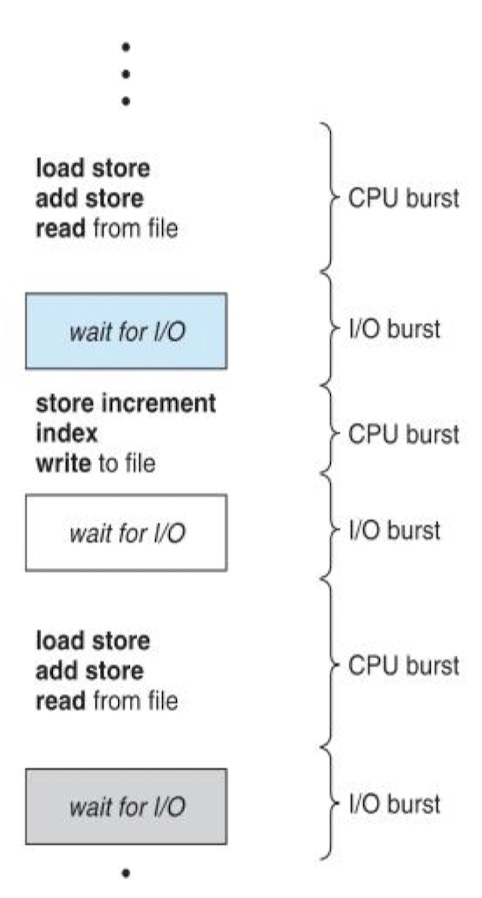
\includegraphics[width=0.22\linewidth]{assets/CPU-IO-burst.jpg}
\end{figure}

Ogni algoritmo di scheduling ha diversi criteri che prova ad ottimizzare, alcuni di questi sono:
\begin{sitemize}
    \item \textbf{Utilizzo della CPU}
    \item \textbf{Throughput:} Numero di processi che completano la loro esecuzione nell'unità di tempo.
    \item \textbf{Tempo di turnaround:} Tempo impiegato per l'esecuzione di un determinato processo
    \item \textbf{Tempo di attesa} nella ready queue
    \item \textbf{Tempo di risposta:} il tempo che intercorre tra una richiesta e una risposta.
\end{sitemize}

\begin{figure}[H]
    \centering
    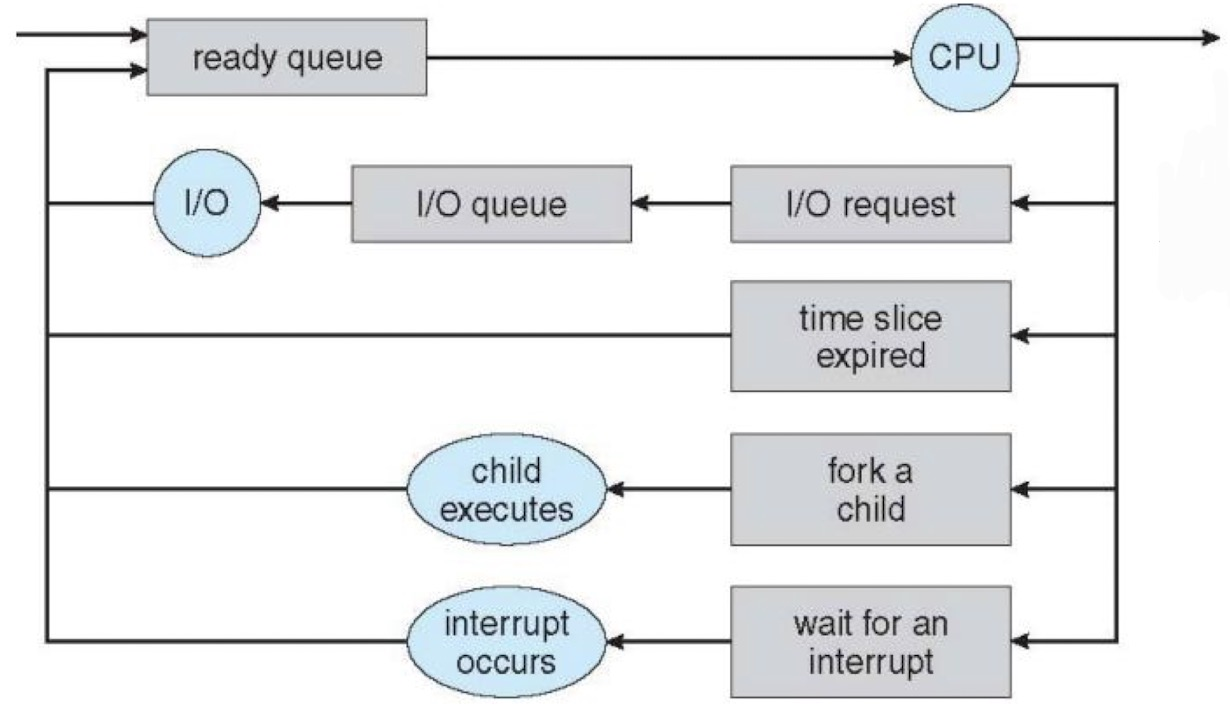
\includegraphics[width=0.5\linewidth]{assets/scheduler.jpg}
    \caption{Diagramma di scheduling}
\end{figure}

\subsection{Meccanismo di Interruzione}
Con \textbf{Meccanismo di Interruzione} intendiamo il meccanismo messo a disposizione dell'elaboratore per salvare lo stato del processo interrotto per poi trasferire il controllo ad una subroutine che gestisce l'interrupt.

\spacer
Il kernel del sistema è composto da 3 sezioni, il \textit{First Interrupt Handler (FLIH)}, il dispatcher e l'implementazione degli strumenti di sincronizzazione.

\subsubsection{First Interrupt Handler}
Il \textit{First Interrupt Handler (FLIH)} ha il compito di determinare l'origine dell'interrupt e attivare il segmento di codice che la gestisce.

\spacer
Nel caso di un sistema che implementa la multiprogrammazione ci possono essere più processi in attesa, è quindi necessario costruire una coda delle interruzioni.

La coda delle interruzioni funziona assieme a la coda dei processi pronti ad eseguire, quando un processo esce dalla coda delle interruzioni viene inserito tra gli altri processi pronti in attesa di risorse computazionali.

\begin{figure}[H]
    \centering
    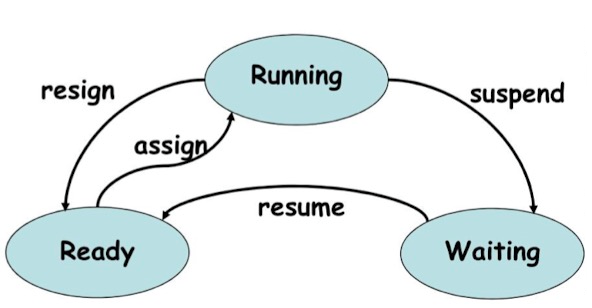
\includegraphics[width=0.45\linewidth]{assets/process-lifecycle.png}
\end{figure}

\subsubsection{Implementazione Strumenti di Sincronizzazione}
Le primitive wait e signal sono implementate dal kernel in quanto possono essere utilizzate da tutti i processi, wait deve poter avere accesso diretto al dispatcher per comunicarci.

\spacer
Ogni semaforo ha una coda, in genere FIFO, che contiene tutti i processi che si sono fermati sul semaforo.

\begin{note}
    Non tutti i semafori sono implementati tramite FIFO, essi in generale possono avere diverse implementazioni e organizzazione.
\end{note}

\subsection{Dispatcher}
Il dispatcher ha il compito di assegnare le risorse di computazione al processo selezionato dallo scheduler. Esso gestisce il context switch tra vari processi.

\begin{figure}[H]
    \centering
    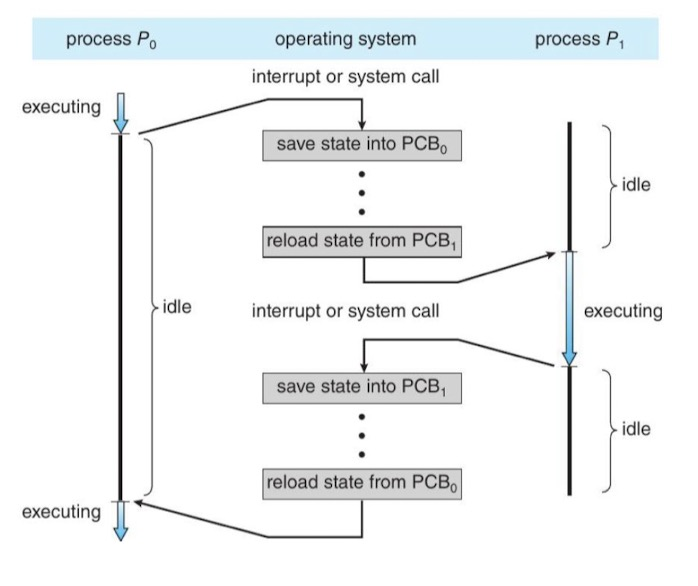
\includegraphics[width=0.5\linewidth]{assets/dispatcher.jpg}
    \caption{Context switch $P_0 \rightarrow P_1 \rightarrow P_0$ }
\end{figure}

Definiamo \textbf{Latenza di dispatch} il tempo impiegato dal dispatcher per scambiare un processo con un'altro. Nello schema qui sopra è il periodo in cui entrambi i processi sono in \textit{idle}.

\subsection{Scheduler ad alto livello}
Il compito di attrubuire il livello di priorità dei processi non è compito del dispatcher, ma dello scheduler di alto livello.

È possibile utilizzare un heap, così da avere buone prestazioni di inserzione ($O(\log_2 n)$) e rendere banale l'estrazione del processo a priorità maggiore.
